\documentclass[12pt]{article}
\usepackage[utf8]{inputenc}
\usepackage[spanish]{babel}
\usepackage[letterpaper]{geometry}
\usepackage{graphicx}
\usepackage{pgfgantt}
\usepackage{listings}
\usepackage{enumitem}
\usepackage{float}
\usepackage{subcaption}
\usepackage{lscape}
\usepackage{geometry}

\usepackage[style=ieee]{biblatex}
\usepackage{csquotes}
\addbibresource{biblio.bib}


\begin{document}

\begin{titlepage}
    \centering
    {
\includegraphics[width=0.2\textwidth]{images/unlp-escudo.png}\par}
    \vspace{1cm}
    {\bfseries\LARGE Universidad Nacional de La Plata \par}
    \vspace{1cm}
    {\scshape\LARGE Facultad de Ingeniería \par}
    \vspace{2cm}
    {\scshape\Huge Cargador de Baterías de Litio de 36V con corriente de salida variable \par}
    \vspace{3cm}
    {\itshape\Large Cátedra de Proyecto Final (E0227) \par}
    \vfill
    {\Large Autores: \par}
    {\large CABRERA, Nicolás \par}
    {\large SÁNCHEZ CROCE, Enzo Imanol \par}
    \vfill
    {\Large 2022 \par}
\end{titlepage}

\newpage

\pagenumbering{arabic}

\begin{abstract}

    El proyecto surge de la necesidad de cargar la batería de una bicicleta eléctrica con asistencia al pedaleo, 
    complementando los proyectos realizados por los alumnos de la cátedra Proyecto Final durante el año 2021.

    Se está desarrollando un cargador para baterías de litio de 36V de diferentes capacidades,
    generalmente utilizadas en vehículos de transporte,
    con la finalidad de ofrecer una carga segura y eficaz.
    El uso de baterías de este tipo está en constante crecimiento y, 
    debido a que el litio es un material altamente reactivo,
    es necesario que el proceso de carga se realice de manera correcta.
    
    En este informe se hará una descripcion de las decisiones tomadas durante la etapa de diseño,
    detallando tanto sobre los avances como los problemas enfrentados,
    junto con las respectivas soluciones propuestas. 

\end{abstract}
\section{Introducción}

El proyecto surge de la necesidad de cargar la batería de litio de una bicicleta eléctrica con asistencia al pedaleo,
complementando los proyectos realizados por los alumnos de la cátedra de Proyecto Final durante el año 2021.
El objetivo principal es diseñar un dispositivo que sea capaz de realizar una carga completa. 

El uso de las baterías de litio está en constante crecimiento y,
debido a que es un material altamente reactivo,
es necesario que el proceso de carga se realice de manera correcta,
con la finalidad de ofrecer una carga segura y eficaz.

El cargador de baterías es un dispositivo electrónico utilizado para suministrar, mediante diferentes etapas, la corriente y tensión continua necesaria para las celdas que componen a una batería recargable, de forma tal que la misma recupere su carga energética.

A continuación se especifican brevemente los contenidos de cada una de las secciones del informe. 
En la sección 2 se introducen los objetivos del proyecto, y en la siguiente se detallan las actividades realizadas y la metodología adoptada para alcanzar las metas y los objetivos propuestos.
En el capítulo 4 se analizan todos los conceptos teóricos necesarios para entender el funcionamiento del cargador y que permiten su desarrollo.
La sección 5 presenta las simulaciones del cargador de baterías de 36V y analiza el modelo de batería utilizado. 
En los capítulos 6 y 7 se introduce el prototipo implementado y se realizan los cálculos necesarios para la elección de cada componente.
La sección 8 detalla todos los criterios aplicados en el diseño del circuito impreso. 
En el capítulo 9 se enumeran los problemas encontrados y las soluciones propuestas durante su implementación. 
La sección 10 presenta las mediciones obtenidas y sus comparaciones con las simulaciones realizadas para el prototipo. 
Finalmente, el último capítulo contiene las conclusiones del proyecto. 
\section{Objetivos}

El objetivo principal de este proyecto es diseñar un dispositivo que sea capaz de realizar una carga completa de una batería 
en buen estado, la cual deberá contar con un sistema de gestión de baterías (BMS, por sus siglas en inglés)
con protección contra sobrecarga, sobre descarga, sobre corriente y temperaturas extremas.

Para lograrlo, el cargador deberá:
\begin{itemize}
    \item Contar con un selector que permita elegir la capacidad de la batería que se desea cargar, regulando de manera acorde la corriente de salida.
    \item Recargar las celdas que componen a la batería, siguiendo un perfil de carga establecido en el proceso de diseño.
    \item Proteger a la batería en caso de un cortocircuito, cortando la alimentación y notificando al usuario mediante el LED indicador.
    \item Garantizar fiabilidad sin generar daños en la batería.
\end{itemize}
\section{Actividades y Metodología}

%Localización física y ubicación de instalaciones:

El proyecto se llevó a cabo en la Facultad de Ingeniería de la Universidad Nacional de La Plata.
Los ensayos necesarios se realizaron en el Área Técnica de Electrónica e Instrumental (ATEI)
del Departamento de Electrotecnia de la Facultad de Ingeniería de la UNLP.
Se realizaron consultas semanales con el tutor para el seguimiento del desarrollo del proyecto y
revisión de las decisiones tomadas por el equipo de trabajo.

Para alcanzar las metas y los objetivos propuestos, se llevaron a cabo las siguientes actividades:

\subsection{Estudio de bibliografía y diseño} \label{subsection:estudio_bibliografia}
Con el objetivo de capacitarse, se estudiaron y analizaron aspectos de seguridad, curvas de carga de la batería 
y topologías de conversores de potencia, de acuerdo con los requerimientos del proyecto. 
Se evaluaron las diferentes alternativas posibles y, en base a su complejidad y a su costo,
se eligió la solución más adecuada para el logro de los objetivos. 

Se realizaron simulaciones en SPICE (programa de simulación con énfasis en circuitos integrados),
separando el proceso en 4 partes:
\begin{itemize}
    \item Fuente conmutada: Convierte la tensión alterna de la red doméstica en una tensión continua.
    \item Fuente de corriente: Brinda una corriente constante a la batería durante la primera etapa de carga.
    \item Circuito de control: Alterna entre las etapas de carga.
    \item Circuito de protección: Protege a la batería en caso de cortocircuito.
\end{itemize}

En la Figura \ref{fig:esquema_cargador} se puede observar un esquema en bloques del cargador.
El circuito de la fuente conmutada está compuesto por los bloques de rectificación, filtrado y conversión DC-DC.
El controlador se encarga de generar una señal PWM en base a la tensión y la corriente de la batería.
La referencia es una señal de corriente ya que la tensión nominal del cargador es fija.
El circuito de protección está integrado en el bloque de control.

Para disminuir las pérdidas de potencia en la etapa de corriente constante y obtener una mayor eficiencia, se modificó la estructura del cargador con respecto al diseño original. 
En primera instancia, para mantener la tensión a la salida del conversor en 42V, se propuso un ciclo de trabajo constante 
con el cual la caída de tensión en la etapa de control de corriente generaba una disipación de potencia excesiva.
Modificando el circuito de conversión que controla tanto la corriente como la tensión se evita una etapa posterior limitadora de corriente.

%incluir esquema de cargador
\begin{figure}
    \centering
    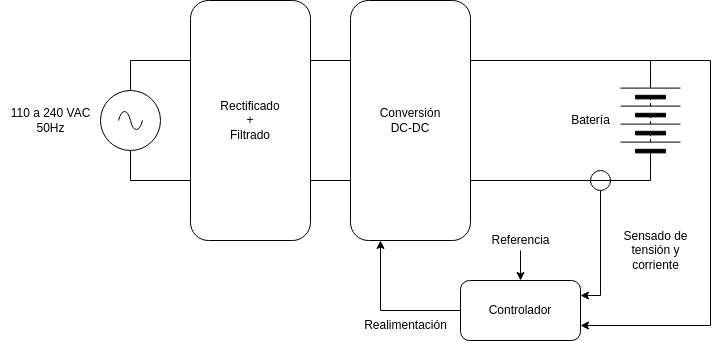
\includegraphics[width=\textwidth]{images/esquema_cargador_v2.png}
    \caption{Esquema del cargador}
    \label{fig:esquema_cargador}
\end{figure}

Se realizó un análisis crítico de las primeras simulaciones y, en base a los resultados obtenidos, 
se corrigieron los circuitos propuestos. 
Esta etapa finaliza con la presentación del informe parcial. 

\subsection{Simulaciones}
El circuito fue diseñado y probado en LTspice \cite{ltspice}, con el fin de verificar el diseño.
El proceso se dividió en las siguientes etapas:
\begin{enumerate}
    \item Simulación del conversor.
    \item Simulación del rectificador de entrada.
    \item Simulación del circuito de control.
    \item Simulación de distintos modelos de batería.
    \item Simulación del driver para el MOSFET high-side.
\end{enumerate}

En las siguientes secciones se detallarán cada una de estas etapas,
enumerando los problemas encontrados y las soluciones propuestas.

\subsubsection{Diseño del conversor}
\marginpar{(Pendiente)}
El primer paso de diseño fue la elección de una topología de conversión DC-DC.
Esta etapa introduce aislación a partir de un transformador de alta frecuencia,
disminuyendo el coste, tamaño y peso respecto a uno de baja frecuencia en base al núcleo magnético necesario.
Como se requiere una única tensión de salida se evita utilizar múltiples devanados.
El conversor debe alcanzar una potencia máxima de 300W y debe ser lo más sencillo posible para evitar un costo elevado. 

La topología flyback es de baja complejidad al estar integrada por muy pocos componentes. 
Como desventajas, el tamaño del núcleo del transformador se incrementa con la potencia requerida y en bornes del
interruptor presenta una tensión igual al doble de la tensión máxima de entrada.
En aplicaciones típicas se alcanzar valores de hasta 150W.

La topología forward con un solo switch disminuye el tamaño del núcleo del transformador ya que la energía no necesita almacenarse en el entrehierro.
Como desventajas, al igual que el flyback presenta alta tensión en bornes del interruptor y se eleva el costo debido al agregado de la bobina de filtrado.
La topología forward con dos switches reduce la tensión en bornes del interruptor a la mitad respecto a la de un solo switch (y con ello la disipación de potencia por switch), 
pero el circuito de excitación de uno de los transistores queda flotante respecto a masa. 
La topología con un solo switch admite una potencia de salida entre 150-250W y con 2 switches se eleva a 500W \cite{mohan}\cite{hart}. 
En base a los criterios definidos inicialmente se eligió el conversor forward con dos switches como topología de conversión DC-DC. 

El principal problema que presentó la utilización de este conversor fue que las señales que controlan a los switches son poco convencionales.

\subsubsection{Simulación del rectificador de entrada AC-DC}
Una vez definido el circuito de conversión DC-DC, se procedió a analizar los requisitos de la tensión de entrada. 
Los circuitos rectificadores AC-DC permiten convertir una tensión alterna en una tensión continua.

\paragraph{Rectificador de media onda u onda completa}

Si bien el rectificador de media onda es más simple ya que cuenta con un menor número de diodos, existen muchas ventajas del rectificador de onda completa frente al de media onda. 
La primera de ellas es que la corriente media del generador de alterna (alimentación) es nula, lo cual beneficia a los transformadores. 
La segunda se basa en el hecho de que para una misma carga,
la tensión de rizado pico a pico para el rectificador de onda completa es
aproximadamente la mitad que para el rectificador de media onda. 
Esto se debe a que en el circuito de onda completa,
el tiempo durante el que se descarga el capacitor es menor que en el circuito de media onda
debido a la onda sinusoidal rectificada de la segunda mitad de cada período. 

Por todos estos motivos se decidió implementar un rectificador de onda completa.

\paragraph{Rectificador de onda completa en puente o con toma media}

\paragraph{En puente}

Presenta la caída de tensión de 2 diodos entre el generador y la carga. 
La tensión máxima en un diodo polarizado en inversa es el valor pico del generador.

\paragraph{Transformador de toma media}

Sólo presenta la caída de tensión de un diodo entre el generador y la carga. 
Para una misma potencia entregada por el generador,
los diodos consumen potencia y disminuyen la corriente y potencia que absorbe la carga. 
La tensión máxima en un diodo polarizado en inversa es el doble del valor pico del generador.
El transformador proporciona aislamiento eléctrico entre el generador y la carga. 

Como la reducción de tensión a la salida no es significativa en esta aplicación
y el puente de diodos se puede implementar con un pequeño integrado,
con el objetivo de disminuir el tamaño del circuito se decidió evitar el transformador
y utilizar un rectificador de onda completa tipo puente.

\paragraph{Filtrado}
% ¿No usamos bobina?
El filtro pasa bajos compuesto por una red LC permite disminuir el rizado,
es decir, la componente de alterna de la señal rectificada. 
Como resultado se logra una tensión de salida aproximadamente continua.
El capacitor mantiene la tensión de salida en un nivel constante y
la bobina suaviza la corriente del rectificador y reduce la corriente de pico en los diodos. 

Para disminuir el número de componentes se decidió utilizar únicamente
un capacitor en paralelo con la capacidad suficiente para obtener una tensión continua.

\paragraph{Rectificación controlada}

Los tiristores son interruptores electrónicos controlados que son activados por una señal externa. 
Poseen 3 terminales: ánodo, cátodo y puerta. Presentan altos valores nominales de corriente y tensión.
Soportan altas corrientes y altas tensiones de bloqueo. 
Un ejemplo de tiristores con los rectificadores controlados de silicio(SCR).
Para que conduzcan se los debe polarizar en directa y deben recibir una corriente de puerta. 
Al entrar en conducción no es necesaria la señal de puerta para mantener la corriente de ánodo. 
El SCR continuará conduciendo siempre que la corriente de ánodo sea positiva y esté por arriba de un valor mínimo. 
Mediante conmutadores controlados como los SCR se controla la tensión de salida en un rango limitado de variación, ajustando el ángulo de disparo de cada SCR. 
El ángulo de disparo es el intervalo angular entre la polarización directa del SCR y la aplicación de la señal de puerta. 
Si el ángulo de disparo es 0, el comportamiento es igual al de un rectificador no controlado con diodos. 

Se decidió utilizar rectificación no controlada ya que no se necesita una tensión específica a la salida
y el costo de complejizar el diseño con el agregado de SCRs y un circuito dedicado de disparo no aporta ningún beneficio significativo.

\subsubsection{Simulación del circuito de control}
Esta etapa fue la mas extensa en diseñar debido a su complejidad.
Inicialmente solo debía realimentar la tensión de salida y generar la señal PWM en base a esta,
pero en base a los cambios descritos en la sección \ref{subsection:estudio_bibliografia}
se separó su diseño en tres etapas:

\begin{enumerate}
    \item Compensador y generador PWM
    \item Selector de modo de funcionamiento
    \item Controlador para los switches
\end{enumerate}

La primer etapa se implementó en base a las topologías descritas en \cite{mohan}. Se puede observar,
en la figura \ref{fig:esquema_compensador}, un modelo simplificado del circuito.

\begin{figure}
    \centering
    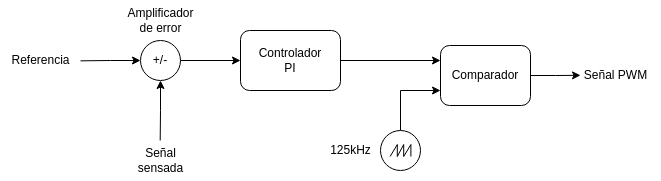
\includegraphics[width=\textwidth]{images/compensador.png}
    \caption{Esquema del compensador y el generador de señal PWM}
    \label{fig:esquema_compensador}
\end{figure}

Los parámetros del bloque proporcional-integrador (PI) fueron definidos a partir de valores típicos obtenidos de \cite{mohan}
y posteriormente ajustados para que el circuito funcione en las condiciones de la aplicación.
La frecuencia de switching es definida por la frecuencia de la señal de diente de sierra y también se tomó un valor típico.

\begin{figure}
    \centering
    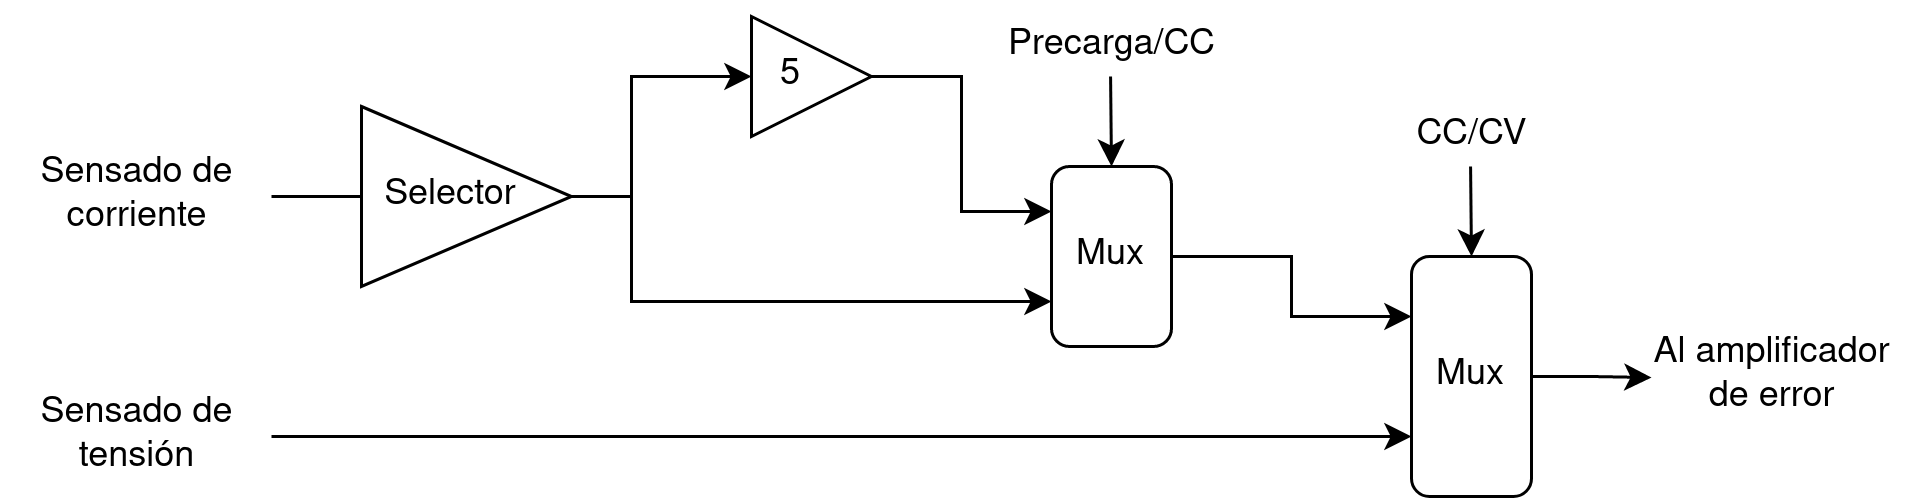
\includegraphics[width=\textwidth]{images/selector.png}
    \caption{Esquema del selector de modo}
    \label{fig:esquema_selector}
\end{figure}

Una vez diseñado el compensador, se procedió a diseñar el circuito de cambio de modo (Precarga, tensión constante y corriente constante).
En la figura \ref{fig:esquema_selector} se puede observar el esquema de este circuito.

Las señales de tensión y corriente están normalizadas con respecto a sus valores nominales.
Un amplificador de ganancia variable actúa como selector de corriente de salida,
modificando la amplitud de la señal de control de dicha variable.
La selección entre el modo de precarga y el modo de corriente constante se hace comparando el nivel de tensión de la batería
con una señal de referencia, siendo el segundo modo activado una vez que la tensión supera los 30V.
El bloque de ganancia 10 tiene como objetivo amplificar la señal de control, ya que la corriente de salida para el modo
de precarga es 10 veces mas chica que la de corriente constante.

La normalización de las señales nombrada anteriormente permite que la selección de la señal del último multiplexor
se haga en base a cual es la mayor de las dos. Esto, visto desde una perspectiva general, permite establecer un límite
tanto de tensión como de corriente de salida, lo cual es importante porque representa la base del método de carga.

Finalmente, para la selección de un controlador para los MOSFETs se tuvieron en cuenta algunos parámetros como
la tensión máxima de entrada, frecuencia de switching y sincronización de las señales,
pero no se logró hallar un controlador adecuado para esta aplicación.
El principal motivo fue que los controladores convencionales generan señales alternadas mediante el método de bootstrapping \cite{hart},
lo cual no sirve para la topología elegida. Esto, combinado con el elevado nivel de tensión en la entrada,
llevó a la búsqueda de otros métodos de control; por eso, se optó por un controlador con transformador aislante para el MOSFET cuyo source no esta a tierra \cite{gatedrivers}. El diagrama de este driver puede observarse en la figura \ref{fig:driver}.

\begin{figure}
    \centering
    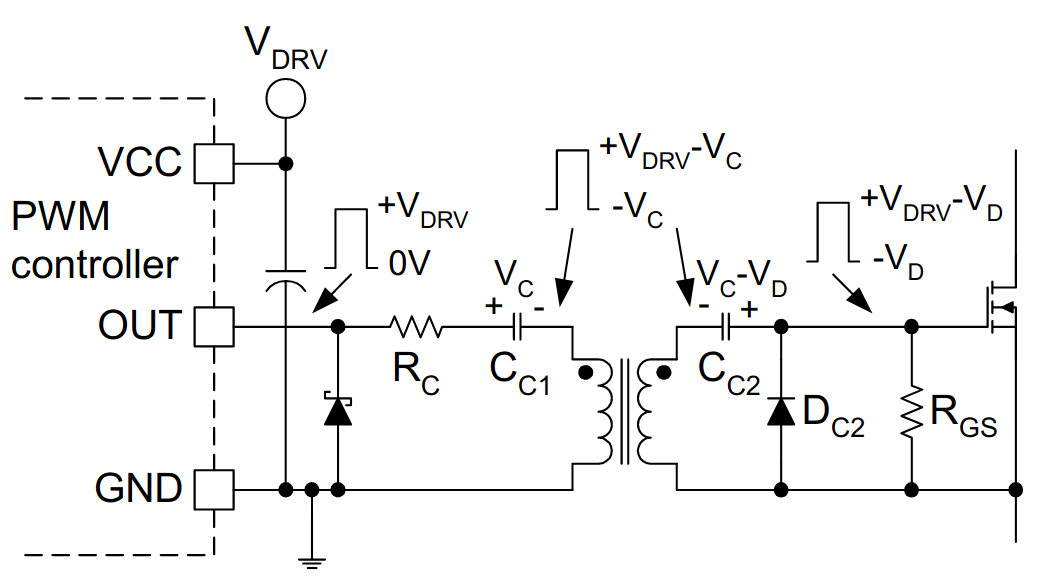
\includegraphics[width=\textwidth]{images/esquema_driver.png}
    \caption{Esquema del controlador del MOSFET high-side}
    \label{fig:driver}
\end{figure}

\subsubsection{Simulación de distintos modelos de batería}
Para que las simulaciones permitan obtener resultados fiables se buscó un modelo apropiado para la batería.
El primer modelo consta de una resistencia variable a partir de los datos obtenidos de los ensayos. 
Este componente representa la resistencia equivalente que presenta la batería,
que es responsable de la caída de tensión instantánea que se produce ante un escalón en la intensidad demandada.

El siguiente modelo propuesto añade un capacitor de muy alto valor en serie con la resistencia variable,
el cual representa la capacidad de almacenar carga de la batería.
El modelo actual es un modelo dinámico donde los valores de los componentes no son fijos,
sino que dependen de las condiciones de funcionamiento de la batería: estado de carga y funcionamiento en carga o descarga.

El circuito de la izquierda modela la resistencia interna de la batería y el comportamiento transitorio ante distintas cargas.
Por otro lado, el circuito de la derecha modela la capacidad de almacenamiento de energía de la batería y la carga almacenada durante los procesos de carga o descarga \cite{modelo_bateria_1}.

\begin{figure}
    \centering
    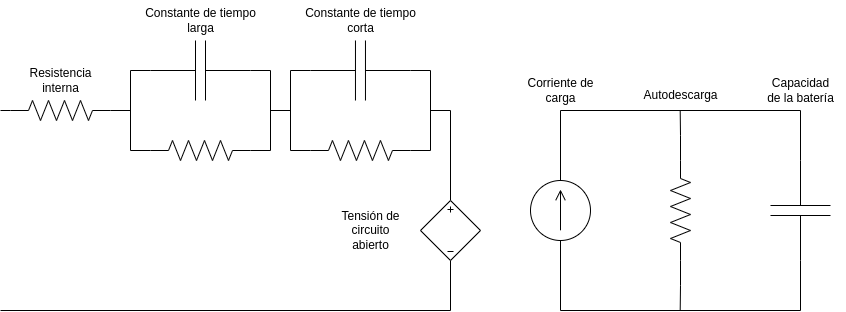
\includegraphics[width=\textwidth]{images/modelo_bateria.png}
    \caption{Modelo final de batería utilizado}
    \label{fig:bateria_3}
\end{figure}

Respecto al segundo modelo se agregan los siguientes componentes:
\begin{itemize}
    \item Los bloques compuestos por una resistencia y un capacitor en paralelo, que modelan la capacidad en los electrodos de las celdas y
    la resistencia no lineal entre electrodos y electrolito.
    En conjunto modelan las constantes de tiempo (corta y larga) de la respuesta transitoria de la tensión en la batería \cite{modelo_bateria_2}.
    \item La fuente de tensión controlada por tensión, que representa la dependencia no lineal entre el estado de carga ($SOC$)
    y la tensión de circuito abierto($V_{OC}$) dependiente del $SOC$.
    \item La fuente de corriente controlada por corriente, representa la corriente de carga que modifica el $SOC$.
\end{itemize}
La tensión que existe en el circuito secundario ($V_{SOC}$) se normaliza de forma que $V_{SOC}=1V$ equivale al $SOC (100\%)$.
La resistencia en paralelo modela la autodescarga de la batería.

\subsection{Implementación}
Se diseñó un circuito impreso y se construyó un prototipo funcional para cumplir con las especificaciones propuestas. 
Debido a que el costo de una batería de litio de las características necesarias es elevado,
se redujo la tensión de salida del conversor a un límite de 12.6V,
tensión que normalmente se utiliza para recargar baterías de computadoras portátiles.

Debido a la extensión del proyecto no se llegó a diseñar el circuito en su totalidad,
por lo que solo se implementó el conversor de tensión continua
junto con el generador de señal PWM y el driver.

Quedó pendiente por implementar todo el circuito de control,
junto con las protecciones necesarias para las baterías.
El rectificador a la entrada del conversor tampoco se llegó a implementar.

\subsection{Validación}
Una vez terminado el proceso de diseño e implementación,
se verificará que el prototipo cumpla con las especificaciones presentadas.

\section{Marco teórico}

Para reducir el tamaño del transformador y cumplir con las especificaciones normalmente se requieren conversiones de etapas múltiples.
Las fuentes de potencia otorgan una alta densidad de potencia en un tamaño y con un peso reducido.  
Permiten aislar eléctricamente a la carga de la red de alimentación. 
Dirección controlada del flujo de potencia. 
Alta eficiencia de conversión. 
Utilizando pequeños filtros es posible tener formas de onda con baja distorsión armónica tanto en la entrada como en la salida. 
Permiten controlar el factor de potencia si la fuente es de AC. 

En base a la tensión de salida requerida existen fuentes de alimentación AC y fuentes de alimentación DC.
Las fuentes de alimentación DC se clasifican en:
1) Conmutación
Tienen una alta eficiencia y pueden suministrar altas corrientes de carga a una tensión baja.
Existen 5 topologías comunes: fly-back, forward, push–pull, half-bridge, y full-bridge.
Por lo general se utilizan 2 etapas de conversión: DC-AC mediante modulación de ancho de pulso (PWM) de la etapa del inversor y de AC-DC.
La salida del inversor, que varía mediante una técnica PWM, se convierte en un voltaje de DC mediante un rectificador de diodos. 
Debido a que el inversor puede operar a una frecuencia muy alta, las fluctuaciones en la tensión de salida de DC se pueden filtrar fácilmente con filtros pequeños. 
2) Resonantes
Si la variación del voltaje de salida no es amplia se pueden usar inversores de pulso resonante. 
La frecuencia del inversor, que podría ser la misma que la frecuencia de resonancia, es muy alta y la tensión de salida del inversor es casi sinusoidal 
Debido a la oscilación resonante, el núcleo del transformador siempre se restablece y no hay problemas de saturación. 
Los tamaños del transformador y del filtro de salida se reducen debido a la alta frecuencia del inversor.
3) Bidireccionales 
Aptas para carga y descarga de baterías donde el flujo de potencia es bidireccional. 
El flujo de potencia depende de la tensión de entrada, de la tensión de salida y de la relación de vueltas del transformador. 
Permiten que la corriente inductiva fluya en cualquier dirección y que el flujo de corriente se vuelve continuo.
Requiere sintetizar las funciones de conmutación para obtener las formas de onda de salida deseadas.

Especificaciones de la tensión de salida del prototipo: 12.6VDC
Para seleccionar una topología adecuada para una aplicación, es necesario comprender las ventajas y desventajas de cada topología y los requisitos de la aplicación. 
Existen diversas topologías, las cuales serán analizadas en orden creciente de complejidad. 
Aunque la mayoría de los convertidores se pueden utilizar para cumplir con los requerimientos de salida, 
los valores nominales del dispositivo de conmutación y el tamaño del transformador limitan sus aplicaciones a una potencia de salida específica. 
La elección del convertidor depende del requisito de potencia de salida y de la complejidad que se desea afrontar.


Conversor Forward


El convertidor forward es un convertidor CC-CC acoplado magnéticamente. 

El transistor funciona como interruptor, estará cerrado un tiempo DT y abierto el resto del tiempo,
 (1 - D)T, siendo T el periodo de conmutación. 
Para el análisis del circuito se supondrá funcionamiento 
en régimen permanente y que la corriente en la inductancia Lx es permanente.
El transformador posee tres devanados: los devanados 1 y 2 transfieren la energía de la
fuente a la carga cuando el interruptor está cerrado; el devanado 3 se usa para proporcionar un
camino a la corriente magnetizante cuando el interruptor está abierto y reducirla a cero antes del
inicio de cada periodo de conmutación. El transformador se modela como tres devanados ideales
con una inductancia magnetizante Lm conectada en paralelo con el devanado 1. En este modelo
de transformador simplificado, no se incluyen las pérdidas ni las inductancias de dispersión.
En el convertidor forward, la energía del generador se transfiere a la carga cuando el interruptor
está cerrado. En el convertidor flyback, la energía se almacenaba en Lm cuando el conmutador
estaba cerrado y era transferida a la carga cuando estaba abierto. En el convertidor directo, Lm
es un parámetro no incluido en la relación entrada-salida, y se suele hacer grande su valor

Análisis con el interruptor cerrado
En la Figura 7.5b se muestra el circuito equivalente del convertidor forward cuando el interruptor
está cerrado. Al cerrarse el interruptor se establece una tensión en el devanado 1 del transformador,
por lo que

La corriente en Lm deberá anularse antes del inicio del siguiente período, para desmagnetizar
el núcleo del transformador. Cuando se abre el interruptor, la Ecuación 7.26 indica que la corriente
iL decrece linealmente. Como D3 impide que la corriente iL se haga negativa, la Ecuación
7.26m será válida siempre que iL sea positiva. Utilizando la Ecuación 7.26 obtenemos



Para que la corriente iL se anule una vez abierto el interruptor, la disminución de corriente
debe ser igual al incremento de la corriente indicado en la Ecuación 7 .20. Si el tiempo necesario
para que la corriente iL de pico se anule es deltaTx, 


Resolviendo para obtener deltaTx, 


El instante t0 en el que se anula la corriente es


Teniendo en cuenta que la corriente debe anularse antes del inicio del siguiente periodo,


Por ejemplo, si la relación N3/N1 = 1, el ciclo de trabajo D deberá ser menor que 0,5. La tensión
en el interruptor abierto es Vs-v1, por lo que


La configuración del circuito a la salida del convertidor forward es la misma que la del convertidor
reductor, por lo que el rizado de la tensión de salida también será el mismo:


Cuando el interruptor está cerrado, la fuente entrega energía a la carga a través del transformador.
La tensión en el secundario del transformador es una forma de onda pulsante y la salida se
analiza de la misma manera que la del convertidor CC-CC reductor. La energía almacenada en
274 Electrónica de potencia
la inductancia magnetizante cuando el interruptor está cerrado puede ser devuelta a la fuente de
entrada a través de un tercer devanado del transformador cuando el interruptor está abierto.

Restablecimiento del núcleo del transformador:
La energía almacenada en el núcleo del transformador es devuelta a la fuente regulable y se incrementa la eficiencia. 

A diferencia del convertidor flyback, la energía no se almacena en el primario y sólo se opera 
en el modo de conducción continua por la mayor dificultad del control en base al doble polo existente en el filtro de salida. 
Asumiendo modo de conducción continua, operación en estado estacionario y ripple de salida nulo, 
existen 2 modos de operación del transistor:

Cuando el transistor se encuentre encendido:

La tensión en el bobinado primario es Vs. La corriente que circula por el mismo comienza a incrementarse 
y se transfiere energía del primario al secundario y de aquí al filtro de salida y la carga por medio del diodo D2. 
Debido a esta corriente se induce una corriente en el secundario dada por:

La corriente magnetizante se incrementa linealmente con el tiempo:

La corriente total que circula por el primario resulta:

Cuando finaliza el tiempo de conducción del transistor en un tiempo t=DT, esta corriente total llega a un valor máximo dado por:

donde XXX es la corriente pico reflejada del inductor de salida del secundario y está dada por:

La tensión inducida en el secundario es:

Debido a la tensión Vsecundario-Vo existente en bornes del inductor, su corriente se incrementa linealmente:

Esta misma también tendrá su valor máximo en t=DT:


Cuando el transistor se encuentre apagado:

La tensión del transformador toma polaridad negativa, lo cual apaga al diodo D2 y enciende a los diodos D1 y D3. 
Mientras conduce D3, la energía es entregada a la carga a través del inductor de salida. 
La corriente por ambos dispositivos es la misma y decrece linealmente con el tiempo:

Lo cual nos da el valor de I1(0):


El diodo D1 y el tercer bobinado del transformador le proporcionan un camino 
a la corriente magnetizante para que regrese a la fuente de entrada. 
La tensión de salida es la integral en el tiempo de la tensión del bobinado secundario:

La máxima corriente de colector se da durante el encendido del transistor y la máxima tensión de colector durante el apagado:


Igualando la integral en el tiempo de la tensión de entrada cuando el transistor está encendido a la tensión Vr cuando el transistor está apagado nos da el ciclo de trabajo máximo:


El ciclo de trabajo debe mantenerse siempre debajo del máximo para evitar la saturación del núcleo del transformador. 
Además, la corriente debe ser reseteada a 0 al final de cada ciclo de conmutación. 
Si el núcleo está saturado, se puede dañar el transistor. 

Comparación con el conversor flyback:

El conversor forward requiere de una carga mínima para evitar un exceso en la tensión de salida. 
Como el transformador no almacena energía, para un mismo nivel de potencia de salida, 
el tamaño del mismo es menor en el convertidor forward que en el flyback. 
La corriente de salida es aproximadamente constante ya que el ripple disminuye notablemente 
debido al agregado del inductor en la salida y al diodo de rueda libre D3.
Por esto mismo, el capacitor de salida puede ser más pequeño. 


Conversor Forward Doble Switch

El conversor forward se utiliza para potencias de salida de hasta 200W ya que se encuentra limitado 
por los esfuerzos de tensión y de corriente durante su funcionamiento. 
El conversor forward de doble switch permite ser utilizado con potencias de hasta X W debido a la 
reducción de la tensión en los transistores cuando los mismos se encuentran apagados. 
Esto permite su uso en aplicaciones de alta tensión mediante transistores de menores prestaciones en tensión. 

Funcionamiento 

Los transistores se encienden y se apagan de forma simultánea. 
Cuando los transistores están encendidos, la tensión en el primario del transformador es igual a la tensión de entrada Vs. 
Como la relación del mismo es 1:1, la misma tensión se establece en su secundario y la energía se transfiere a la carga. 
Además se incrementa la corriente que circula por la inductancia magnetizante. 

Cuando los transistores se apagan, el diodo D1 evita que la corriente magnetizante circule por el secundario 
(y por lo tanto también en el primario) del transformador, forzando su camino por los diodos D3 y D4 de regreso a la fuente regulable.  
Con esto se elimina la necesidad del tercer devanado de desmagnetización. 
La tensión en el primario del transformador es -Vs, causando un decremento de la corriente magnetizante. 
Si la relación de trabajo de los transistores es menor a 0.5, en cada ciclo el núcleo del transformador se restablece, 
haciendo que el flujo magnético regrese a 0. 
La tensión en los transistores cuando los mismos se encuentran apagados es Vs y no Vs(1+N1/N3).

La tensión de salida resulta:
$$ V_{o}=V_{s}D(\frac{N_{2}}{N_{1}}) $$




Circuitos de control

La tensión de salida del convertidor puede ser controlada variando el ciclo de trabajo D. 
Para ello se utilizan controladores de circuito integrado PWM que sólo requieren de unos pocos componentes pasivos adicionales para su funcionamiento. 
Internamente presenta 4 componentes principales:
1) Un reloj ajustable que permite configurar la frecuencia de conmutación 
2) Amplificador de error para la tensión de salida
3) Generador de forma de onda de dientes de sierra sincronizado con el reloj
4) Un comparador para comparar la señal de salida de error con la señal de dientes de sierra.
Su señal de salida es la que controla a los transistores. 

Para controlar la tensión de salida, los convertidores funcionan con un circuito de retroalimentación,
 en base a la señal realimentada , en un control por tensión o corriente.

Control por tensión

COMPLETAR CON LIBRO

La duración del tiempo de encendido está determinada por el tiempo entre el reinicio del generador de diente de sierra
 y la intersección del voltaje de error con la señal de rampa positiva. 
 Cuando la tensión de salida es inferior al valor nominal se genera una tensión de error. 
 El ciclo de trabajo aumenta para causar un aumento posterior en el voltaje de salida. 
 La dinámica de retroalimentación está determinada por el circuito amplificador de error que consta de Z1 y Z2.



 Control por corriente 

 Consiste en un lazo interno que muestrea el valor de la corriente primaria y apaga los interruptores tan pronto como la corriente alcanza cierto valor establecido por el lazo de voltaje externo. 
 De esta manera, el control de corriente logra una respuesta más rápida que el modo de voltaje. 
 La forma de onda de corriente primaria actúa como onda de diente de sierra. 
 El voltaje análogo a la corriente puede ser proporcionado por una pequeña resistencia o por un transformador de corriente. 
 La figura 13.19a muestra un convertidor flyback controlado por modo de corriente, donde la corriente del interruptor isw se usa como señal portadora. 
 La corriente del interruptor isw produce un voltaje a través de Rs, que se retroalimenta al comparador. 
 El encendido está sincronizado con el pulso del reloj y el apagado está determinado por el instante en que la corriente de entrada es igual al voltaje de error.
 Debido a su capacidad inherente de limitación de corriente máxima, el control de modo de corriente puede mejorar la confiabilidad de los interruptores de alimentación. El rendimiento dinámico se mejora debido al uso de la información actual adicional. El control de modo de corriente reduce efectivamente el sistema a primer orden al obligar a que la corriente del inductor se relacione con el voltaje de salida, logrando así una respuesta más rápida. Las figuras 13.18b–e muestran las formas de onda.

 COMPLETAR CON JUSTIFICACIÓN DE POR QUÉ NO ELEGIMOS CONTROL POR CORRIENTE QUE PARECERÍA SER MEJOR. 


 
\input{sections/diseño.tex}
\section{Driver}

Los MOSFET se encargan de conectar la alimentación con la carga. El IRF840 es un MOSFET de canal N. 
Para encenderlo se debe aplicar una tensión positiva entre Gate y Source. 
Debido a la configuración de convertidor elegida, se requiere un driver para controlar el MOSFET cuyo terminal de \textit{source} no está a tierra. Se optó por un driver con transformador acoplador ya que provee aislación galvánica entre el circuito de control y el circuito de potencia \cite{gatedrivers}.

Existen 2 posibles configuraciones para un transistor según su posición en el circuito:

Low side: utiliza comúnmente el MOSFET de canal N. 
El terminal Source está a tierra y la carga se encuentra entre la alimentación y el terminal Drain. 
Mientras está encendido le otorga a la carga el camino hacia la tierra y cuando está apagado se sitúa debajo de la misma. 

High Side: utiliza comúnmente el MOSFET de canal P. 
El terminal Drain se encuentra conectado a la alimentación y el terminal Source a la carga. 

% INSERTAR FIGURA DE GOOGLE!

Para controlar high side MOSFETs se puede utilizar un circuito integrado o un transformador. 
Los circuitos integrados, si bien son más pequeños y ocupan menor espacio en las placas, 
poseen tiempos significativos de encendido y apagado. 
El transformador es de un tamaño mucho mayor, requiere de un diseño apropiado y de componentes adicionales,
 pero sus tiempos de encendido y apagado son despreciables y permite operar con diferencias de tensión más elevadas.

Los transformadores poseen al menos 2 bobinados acoplados magnéticamente, 
lo cual permite generar aislación entre el circuito primario y secundario. 
La relación de vueltas entre los mismos permite modificar la tensión de salida obtenida. 
Los transformadores manejan muy poca potencia promedio, pero entregan altos picos de corriente en el encendido y apagado.

Si bien el transformador ideal no almacena energía, los transformadores reales 
almacenan una pequeña cantidad de energía entre los bobinados y los posibles huecos de aire presentes en el mismo. 
Esto se representa mediante una inductancia magnetizante. 
Una pequeña inductancia minimiza la energía almacenada permitiendo aumentar la eficiencia y disminuye los retrasos de tiempo. 

Para cumplir con la ley de Faraday, la tensión en la bobina del transformador debe ser nula en una parte del período, 
por lo cual cualquier pequeña señal de continua puede hacer saturar al núcleo. 
La saturación limita el producto volt-segundo aplicado a través de los devanados. 
Su valor máximo se da en la peor condición de funcionamiento con el ciclo de trabajo máximo y la tensión de entrada máxima simultáneamente. 

Como el convertidor forward trabaja sólo en el primer cuadrante del plano B-H, una gran parte del período de switching debe reservarse para restaurar el núcleo de la potencia del transformador. 
Esto limita la relación de trabajo del transformador, pero no suele ser un problema ya que 
el transformador debe estar acoplado a corriente alterna y por lo tanto funciona con magnetización bidireccional. 

La figura X muestra el circuito básico del driver mediante un transformador. 

INSERTAR FIGURA 33: Single-Ended Transformer-Coupled Gate Drive

A continuación se detalla información relevante de cada componente: 

1)Entrada single-ended de un controlador PWM.

2) Capacitor de acoplamiento Cc1

Para evitar la componente continua se coloca un capacitor de acoplamiento en serie con el bobinado primario, 
evitando la saturación del núcleo. La tensión sobre el mismo resulta: 

Vcc1=D*Vdrv

En base al máximo ripple de tensión permitido y la carga que atraviesa a los capacitores de acoplamiento en estado estacionario:

INSERTAR FÓRMULA DE CC1

Para este capacitor, el ripple tiene una componente relacionada a la carga del MOSFET, 
otra relacionada con la corriente que pasa por la resistencia entre Gate y Source 
y una última componente relacionada a la corriente de la inductancia magnetizante. 
La capacidad es máxima para un ciclo de trabajo determinado definido por los parámetros de diseño 
y los valores de los componentes y se obtiene derivando a la expresión en función del ciclo. 

Constante de tiempo de la tensión en el capacitor de acoplamiento:

INSERTAR FÓRMULA

Para anchos pulsos del ciclo de trabajo, se requieren de componentes adicionales 
en el secundario del transformador para proveer de la tensión correcta al Gate. 
La tensión a través del capacitor de acoplamiento se incrementa de forma proporcional al pulso. 
La tensión negativa durante el tiempo que está apagado aumenta y la tensión positiva durante el tiempo que está encendido disminuye. 

INSERTAR FORMA DE ONDA SOBRE EL CAPACITOR (SE SACA DEL ESQUEMÁTICO DADO)

3) Resistencia de amortiguamiento Rc

Cambios repentinos en el ciclo de trabajo excitan a la red LC compuesta por el capacitor de acoplamiento 
y la inductancia magnetizante, provocando resonancias indeseadas en la tensión sobre el capacitor. 
Esta resistencia de bajo valor en serie con el capacitor de acoplamiento permite amortiguar las resonancias. 

Rc>=2*sqrt(Lm/Cc1)

Si la resistencia es muy grande, genera una sobre amortiguación que limita la corriente que ingresa al terminal Gate y disminuye la frecuencia de switching. 
Si la resistencia es muy chica, las resonancias provocadas generan una tensión entre Gate y Source muy elevada.

4) Resistencia de carga entre Gate y Source Rgs

Resistencia de pull down: Pone a tierra el terminal Gate al alimentar el circuito, manteniendo al MOSFET apagado durante el inicio. 
Además le provee de un camino para la corriente que circula por el capacitor de acoplamiento, 
permitiendo establecer la tensión necesaria sobre el mismo y que en cada ciclo de switching 
la misma carga del Gate sea entregada y removida a través del capacitor. 

5) Diodo Schottky 

Debido a la componente de corriente de la inductancia magnetizante, la salida debe manejar corriente de forma bidireccional. 
Por ello se requiere un diodo Schottky a la entrada. 
El mismo puede evitarse aumentando la componente de corriente resistiva para contrarrestar a la componente de la inductancia magnetizante. 

6) Capacitor de acoplamiento Cc2  

Se agrega un segundo capacitor de acoplamiento que permite restaurar a los niveles originales de tensión. 
El agregado opcional de un diodo zener en serie permite incremetar aún más la tensión negativa durante el apagado. 

En base al máximo ripple de tensión permitido y la carga que atraviesa a los capacitores de acoplamiento en estado estacionario:

INSERTAR FÓRMULA DE CC2 
CORREGIR DE LA FÓRMULA: ES VDRV Y NO VDRC

Para este capacitor, el ripple tiene una componente relacionada a la carga del MOSFET 
y otra relacionada con la corriente que pasa por la resistencia entre Gate y Source. 
La capacidad es máxima cuando el ciclo de trabajo es máximo. 

7) Diodo clamp

Evita sobre tensiones.


Diseño del transformador:

Su diseño es similar a un transformador de potencia. 
Su función es transmitir el pulso de accionamiento de puerta referenciado a tierra a través de grandes diferencias de potencial para adaptarse a las implementaciones de accionamiento flotante. Para hacerlo maneja muy poca potencia pero requiere de elevados picos de corriente. 

Su relación será 1:1 ya que no se requiere.......

Está controlado por un ancho de pulso variable y de amplitud constante.

Está acoplado a CA y la inductancia de magnetización ve un pulso de amplitud variable.

Operan en el primer y tercer cuadrante del plano B-H.

Primero se selecciona el núcleo. En base a la disponibilidad se elige el E25. 
El material del núcleo es ferrita de alta permeabilidad para maximizar el valor de 
la inductancia de magnetización y, en consecuencia, reducir la corriente de magnetización.

Número de vueltas del primario: 

INSERTAR FÓRMULA DEL NÚMERO DE VUELTAS JUNTO A LA DESCRIPCIÓN DE CADA variable

Primero se halla el numerador con:

INSERTAR IMÁGEN 36: Gate-Drive Transformer Volt-second Product vs. Duty Ratio

Para un circuito acoplado de CA, el peor de los casos es D = 0,5, 
mientras que el acoplamiento directo alcanza el valor pico de voltios por segundo en la máxima relación de trabajo operativa. 
Curiosamente, el acoplamiento de CA reduce el producto volt-segundo de estado estacionario máximo en un factor de cuatro debido a que, 
en relaciones de trabajo grandes, el voltaje del transformador se reduce proporcionalmente debido al voltaje que 
se desarrolla a través del capacitor de acoplamiento.
Delta B: valor pico a pico del cambio en el flujo que se produce durante la duración del pulso. 

Es mucho más difícil calcular $\Delta B$ en la ecuación Np. 
La razón es el desplazamiento del flujo durante el funcionamiento transitorio. 
Cuando el voltaje de entrada o la carga cambian rápidamente, el controlador PWM ajusta la relación de trabajo en consecuencia. 
Es bastante difícil deducir el resultado cuantitativo exacto de la caminata de flujo. 
Depende de la respuesta del lazo de control y de la constante de tiempo de la red de acoplamiento cuando está presente. 
En general, una respuesta de bucle más lenta y una constante de tiempo más rápida tienden a reducir el desplazamiento de flujo. 
Para la mayoría de los diseños, es deseable un margen de tres a uno entre la densidad de flujo de saturación 
y el valor de flujo máximo en el peor de los casos de operación en estado estable para cubrir la operación transitoria.

\section{Simulaciones}

% 1) Tensión de salida en el colector del TL494
% 2) Tensión en el capacitor Ct
% 3) Tensión de salida de la etapa de ganancia de corriente
% 4) Tensión en el primario del transformador del driver
% 5) Tensión en el secundario del transformador del driver
% 6) Corriente en el primario del transformador del driver
% 7) Corriente en la resistencia entre gate y source del driver
% 8) Corriente que circula por el gate del MOSFET 1 (high side)
% 9) Corriente que circula por el gate del MOSFET 2 (low side)
% 10) Corriente que circula por el drain del MOSFET 1 (high side)
% 11) Corriente que circula por el drain del MOSFET 2 (low side)
% 12) Corriente en el primario del transformador de potencia 
% 13) Corriente en el inductor del filtro de salida 
% 14) Corriente por la carga y su ripple
% 15) Tensión entre gate y source del MOSFET 1 (high side)
% 16) Tensión entre drain y source del MOSFET 1 (high side)
% 17) Tensión entre gate y source del MOSFET 2 (low side)
% 18) Tensión entre drain y source del MOSFET 2 (low side)
% 19) Tensión en el primario del transformador de potencia 
% 20) Tensión en el secundario del transformador de potencia 
% 21) Tensión de salida sobre la carga y su ripple 
% 22) Tensión en el inductor del filtro de salida
% 23) Corriente de salida por colector del TL494 
% 24) Tensión cátodo ánodo en el diodo D1
% 25) Tensión cátodo ánodo en el diodo D2
% 26) Tensión cátodo ánodo en el diodo D3
% 27) Tensión cátodo ánodo en el diodo D4
% 28) Corriente en el secundario del transformador de potencia

En esta sección se comparan las formas de onda obtenidas con el circuito una vez implementado, con las simulaciones realizadas para el diseño del cargador de baterías.

\subsection{Generador de señal PWM}

Por cuestiones de costo computacional y de falta de un modelo representativo del TL494,
su circuito no fue simulado y se probó directamente en una protoboard,
por lo que no se harán comparaciones con las simulaciones.

Aun así, a continuación se mostrarán las formas de onda mas importantes del circuito implementado,
comparando con las indicadas en la hoja de datos del fabricante.

En la figura \ref{fig:osc_pwm_vout_disconnected} se muestra la forma de onda de la tensión de salida de la etapa de ganancia de corriente, con la fuente de alimentación de 36V desconectada.
Esta debería ser una señal PWM con un período de $8\mu s$ y un ancho de pulso de aproximadamente 16\%

\begin{figure}[H]
    \centering
    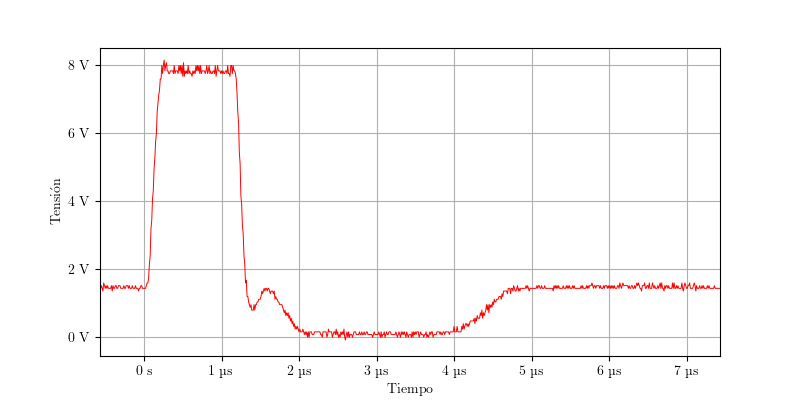
\includegraphics[width=\textwidth]{images/capturas-osciloscopio/TL494/pwm_vout_disconnected.png}
    \caption{Tensión a la salida del TL494 después de la etapa de ganancia de corriente con la fuente de 36V desconectada. Se puede observar que la señal cumple con los requisitos de frecuencia y ancho de pulso}
    \label{fig:osc_pwm_vout_disconnected}
\end{figure}

Se puede observar una tensión de continua de aproximadamente $1.5V$ durante la etapa de apagado del PWM, la cual se debe al capacitor de desacople del circuito primario del driver.

Si se compara la figura \ref{fig:osc_pwm_vout_disconnected} con la \ref{fig:osc_pwm_vout_connected}, la cual muestra la misma forma de onda pero con la fuente de tensión de 36V conectada, se puede observar que la forma de onda es similar, pero se presenta una oscilación de alta frecuencia durante el ciclo de apagado de la señal PWM. Esta oscilación será tratada en la sección %\ref{subsec:oscilaciones}.

\begin{figure}[H]
    \centering
    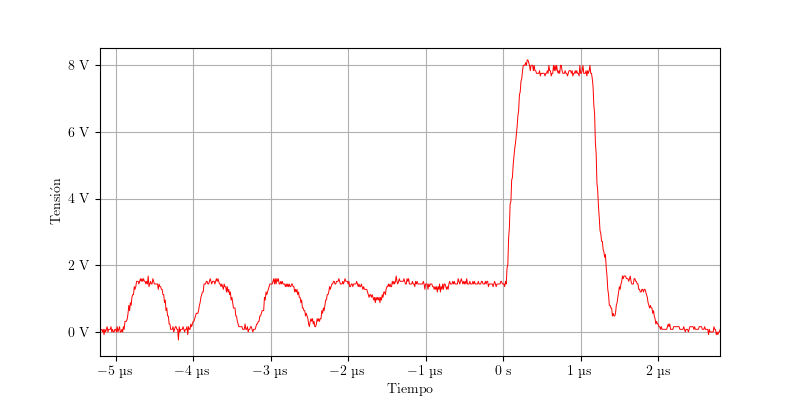
\includegraphics[width=\textwidth]{images/capturas-osciloscopio/TL494/pwm_vout_connected.png}
    \caption{Tensión a la salida del TL494 después de la etapa de ganancia de corriente con la fuente de 36V conectada}
    \label{fig:osc_pwm_vout_connected}
\end{figure}

En las figuras \ref{fig:ct_v} y \ref{fig:dtc_v} se muestran las tensiones en el capacitor $C_t$ y el terminal DTC del TL494 respectivamente.

\begin{figure}[H]
    \centering
    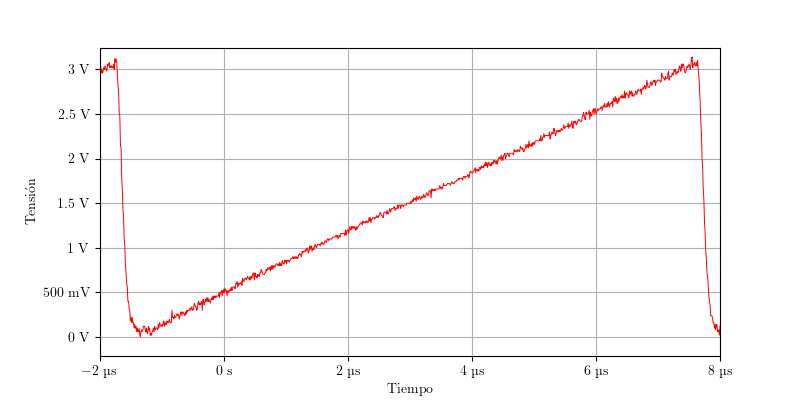
\includegraphics[width=\textwidth]{images/capturas-osciloscopio/TL494/Ct_v.png}
    \caption{} %COMPLETAR
    \label{fig:ct_v}
\end{figure}

% La forma de onda de Ct es la esperada, pero la de DTC?

\begin{figure}[H]
    \centering
    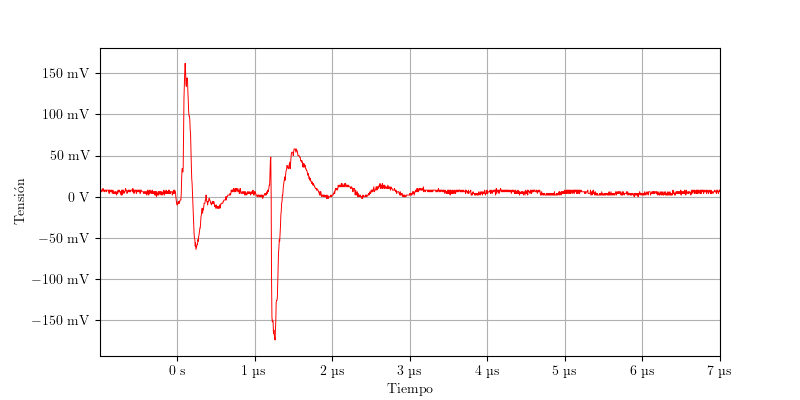
\includegraphics[width=\textwidth]{images/capturas-osciloscopio/TL494/DTC_v.png}
    \caption{} %COMPLETAR
    \label{fig:dtc_v}
\end{figure}

% 1) Señal PWM

% Se toma la salida por el colector de los transistores del circuito integrado. 
% Su forma de onda son pulsos rectangulares. 
% Amplitud: 0V a Vdrv dados por la tensión de alimentación.
% Frecuencia de 125kHz dada por el capacitor Ct=1nF y $Rt=8k\Omega$ mediante el potenciómetro. 
% Tiempo de encendido: permite controlar el ciclo de trabajo mediante un potenciómetro. 
% Esta señal se mide en 3 condiciones diferentes: 
% A) Sin el convertidor forward conectado
% B) Con el convertidor forward conectado pero sin su alimentación de 36V
% C) Con el convertidor forward conectado y alimentado

% 2) Diente de Sierra 

% Tensión en el capacitor Ct. 

% 3) Tensión en el puerto DTC 

\subsection{Etapa de ganancia de corriente}

En las figuras \ref{fig:pwm_iout_sin_bjt} y \ref{fig:pwm_iout_con_bjt} puede observarse la corriente de salida del TL494 antes y después de agregar la etapa de ganancia de corriente, respectivamente.

\begin{figure}[H]
    \centering
    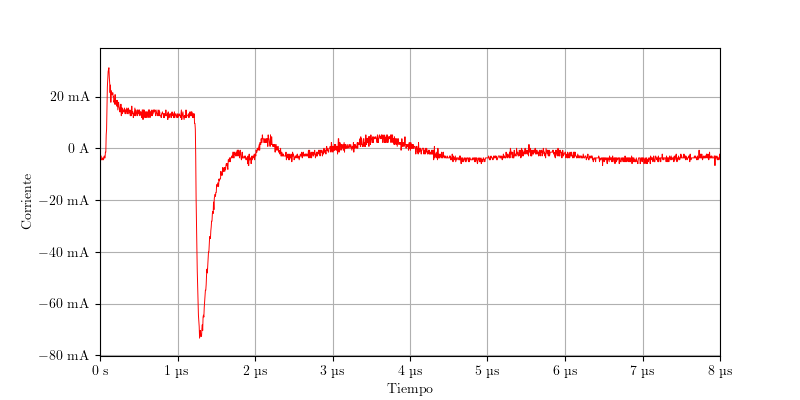
\includegraphics[width=\textwidth]{images/capturas-osciloscopio/TL494/pwm_iout_sin_bjt.png}
    \caption{Corriente a la salida del TL494 sin colocar la etapa intermedia de ganancia de corriente}
    \label{fig:pwm_iout_sin_bjt}
\end{figure}

\begin{figure}[H]
    \centering
    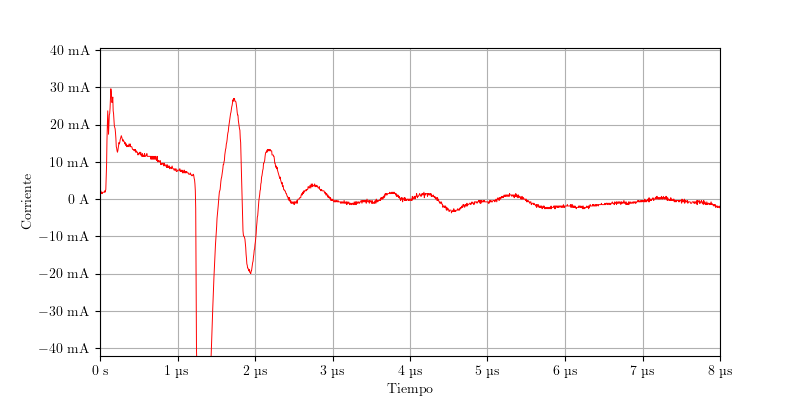
\includegraphics[width=\textwidth]{images/capturas-osciloscopio/BJT/bjt-iin-con-etapa.png}
    \caption{Corriente a la salida del TL494 con la etapa intermedia de ganancia de corriente}
    \label{fig:pwm_iout_con_bjt}
\end{figure}

Puede observarse que las oscilaciones aumentan. %WHAT?

La funcion más importante de esta etapa es la de mejorar la forma de onda de la señal PWM, que al comparar las figuras \ref{fig:osc_pwm_vout_disconnected} y \ref{fig:pwm_vout_sin_bjt} se puede observar que se ha mejorado considerablemente.

\begin{figure}[H]
    \centering
    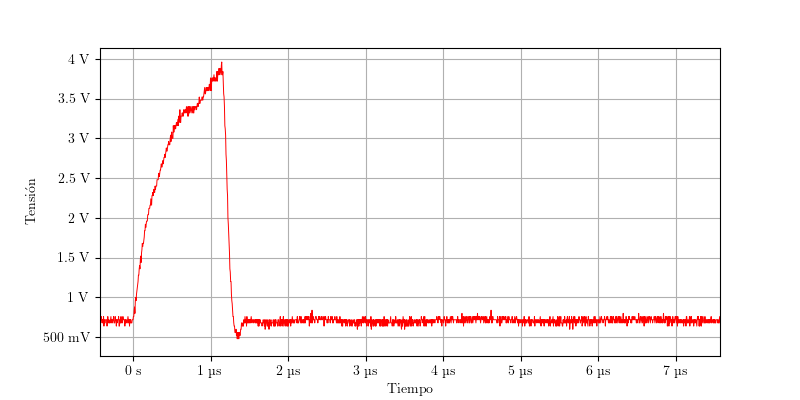
\includegraphics[width=\textwidth]{images/capturas-osciloscopio/TL494/pwm_vout_sin_bjt.png}
    \caption{Tensión a la salida del TL494 sin colocar la etapa intermedia de ganancia de corriente}
    \label{fig:pwm_vout_sin_bjt}
\end{figure}

% 1) Corriente sin la etapa 
% DONE

% 2) Corriente de entrada y de salida con la etapa

% 3) Tensión a la salida sin la etapa
% DONE

% 3) Tensión a la salida con la etapa
% DONE

% Hay que ver eso de las oscilaciones en la corriente

\subsection{Driver}

En las figuras \ref{fig:driver_vout_connected} y \ref{fig:driver_vout_disconnected} se muestra la salida del driver con y sin el convertidor energizado, respectivamente.
Se puede ver que también están presentes las oscilaciones de alta frecuencia que se observan en la salida del TL494.

\begin{figure}[H]
    \centering
    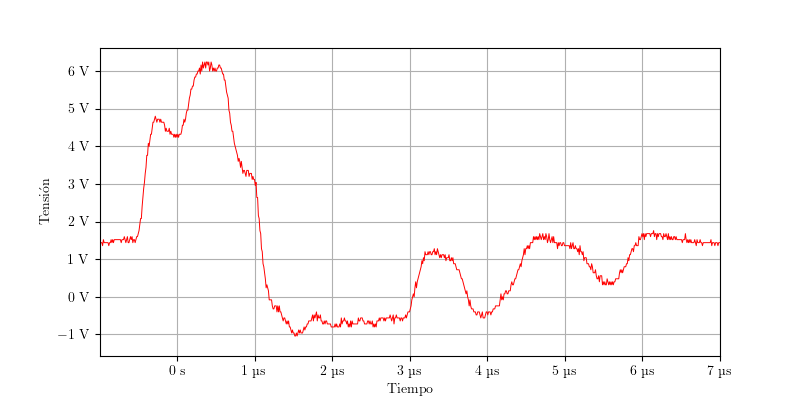
\includegraphics[width=\textwidth]{images/capturas-osciloscopio/DRIVER/driver_vout_connected.png}
    \caption{Tensión a la salida del driver con la fuente de 36V conectada}
    \label{fig:driver_vout_connected}
\end{figure}
% HAY QUE ORDENAR ESTAS 2
\begin{figure}[H]
    \centering
    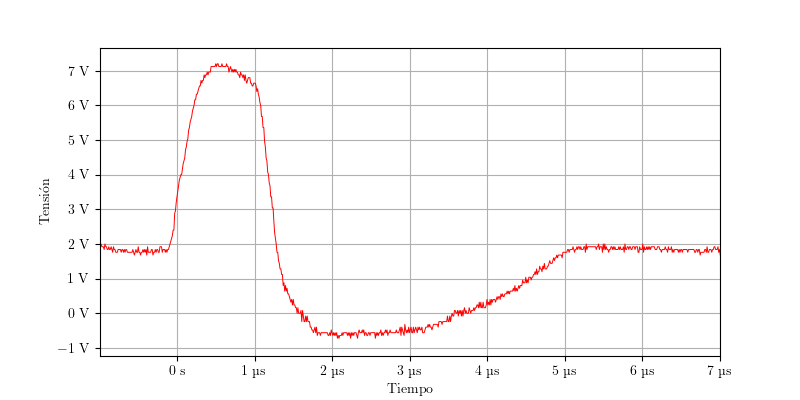
\includegraphics[width=\textwidth]{images/capturas-osciloscopio/DRIVER/driver_vout_disconnected.png}
    \caption{Tensión a la salida del driver con la fuente de 36V desconectada}
    \label{fig:driver_vout_disconnected}
\end{figure}

En la figura \ref{fig:driver_expected_waveforms} se muestran algunas formas de onda del circuito del driver con las que se hicieron comparaciones para verificar su correcto funcionamiento.

\begin{figure}[H]
    \centering
    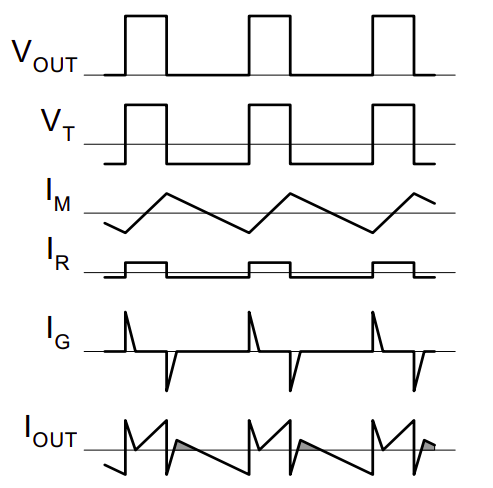
\includegraphics[width=0.7\textwidth]{images/driver_expected_waveforms.png}
    \caption{Formas de onda esperadas de distintas señales del driver \cite{gatedrivers}}
    \label{fig:driver_expected_waveforms}
\end{figure}

%Falto medir la mayoría de esto?
% 1) Tensiones en el transformador de señal 

    % Forma de onda: Rectangular 
    % Amplitud: -Vc a Vdrv-Vc 
    % Son iguales dada la relación 1:1 del transformador. 

% 2) Tensión Gate del MOSFET high side % Sería vout del driver?
% DONE

    % Forma de onda: Rectangular 
    % Amplitud: -Vd a Vdrv-Vd
    % Vd: Tensión en el diodo del secundario

% 3) Corriente de salida % FALTA MEDIR LAS CORRIENTES CON LA PCB

    % Compuesta por:

    % A) Corriente magnetizante

        % Forma de onda: triangular
        % Se mide en la Rc del primario. 

    % B) Corriente por Rgs

        % Forma de onda: rectangular

    % C) Corriente por Gate

        % Forma de onda: diente de sierra invertida y espejada con tiempo muerto 

\subsection{Convertidor Forward Doble Switch}

% Agregar intro

% 1) Vgs de ambos MOSFETs %Ya se midió en otros lados

% 2) Vds de ambos MOSFETs

En las figuras \ref{fig:vds_high} y \ref{fig:vds_low} se muestran las tensiones en los terminales \textit{drain} y \textit{source} de los MOSFETs del convertidor forward doble switch.
Para comparar, se muestra en la figura \ref{fig:vds_simulation} la tensión $V_{DS}$ del MOSFET low side simulada en LTSpice. Idealmente, las formas de onda en ambos transistores son iguales.

\begin{figure}[H]
    \centering
    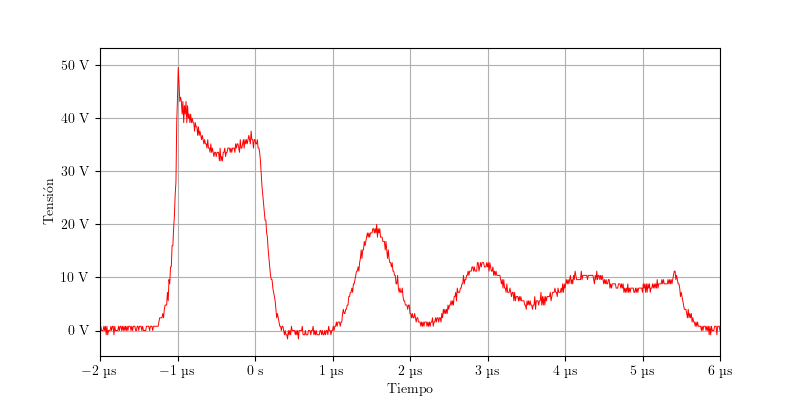
\includegraphics[width=0.7\textwidth]{images/capturas-osciloscopio/MOSFET/vds-high.png}
    \caption{Tensión $V_{DS}$ en el MOSFET high side}
    \label{fig:vds_high}
\end{figure}

\begin{figure}[H]
    \centering
    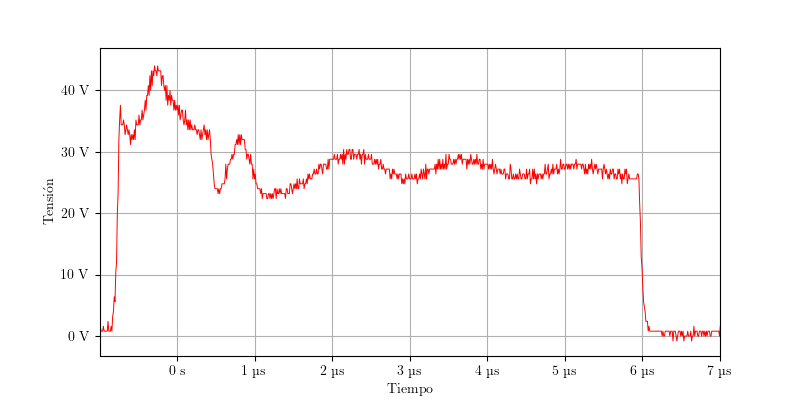
\includegraphics[width=0.7\textwidth]{images/capturas-osciloscopio/MOSFET/vds-low.png}
    \caption{Tensión $V_{DS}$ en el MOSFET low side}
    \label{fig:vds_low}
\end{figure}

% \begin{figure}[H]
%     \centering
%     \includegraphics[width=0.7\textwidth]{images/vds_sim.png}
%     \caption{Tensión $V_{DS}$ en el MOSFET low side simulado en LTspice}
%     \label{fig:vds_low}
% \end{figure}

% 3) Idrain de ambos MOSFETs

% 4) Tensiones en el E70

% 5) Corriente en el primario

    % Medir la componente continua. 

% 6) Caída de tensión en los diodos

% 7) Corriente en el inductor junto con su ripple

% 8) Corriente de salida junto con su ripple 

    % Idealmente medir 1A-1.6A del modo elegido. 

% 9) Tensión de salida junto con su ripple 

\subsubsection{Simulación de distintos modelos de batería}
Para que las simulaciones permitan obtener resultados fiables se buscó un modelo apropiado para la batería.
El primer modelo consta de una resistencia variable a partir de los datos obtenidos de los ensayos. 
Este componente representa la resistencia equivalente que presenta la batería,
que es responsable de la caída de tensión instantánea que se produce ante un escalón en la intensidad demandada.

El siguiente modelo propuesto añade un capacitor de muy alto valor en serie con la resistencia variable,
el cual representa la capacidad de almacenar carga de la batería.
El modelo actual es un modelo dinámico donde los valores de los componentes no son fijos,
sino que dependen de las condiciones de funcionamiento de la batería: estado de carga y funcionamiento en carga o descarga.

El circuito de la izquierda modela la resistencia interna de la batería y el comportamiento transitorio ante distintas cargas.
Por otro lado, el circuito de la derecha modela la capacidad de almacenamiento de energía de la batería y la carga almacenada durante los procesos de carga o descarga \cite{modelo_bateria_1}.

\begin{figure}
    \centering
    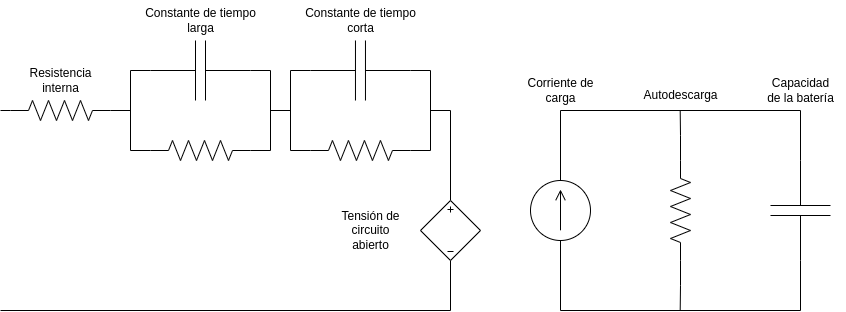
\includegraphics[width=\textwidth]{images/modelo_bateria.png}
    \caption{Modelo final de batería utilizado}
    \label{fig:bateria_3}
\end{figure}

Respecto al segundo modelo se agregan los siguientes componentes:
\begin{itemize}
    \item Los bloques compuestos por una resistencia y un capacitor en paralelo, que modelan la capacidad en los electrodos de las celdas y
    la resistencia no lineal entre electrodos y electrolito.
    En conjunto modelan las constantes de tiempo (corta y larga) de la respuesta transitoria de la tensión en la batería \cite{modelo_bateria_2}.
    \item La fuente de tensión controlada por tensión, que representa la dependencia no lineal entre el estado de carga ($SOC$)
    y la tensión de circuito abierto($V_{OC}$) dependiente del $SOC$.
    \item La fuente de corriente controlada por corriente, representa la corriente de carga que modifica el $SOC$.
\end{itemize}
La tensión que existe en el circuito secundario ($V_{SOC}$) se normaliza de forma que $V_{SOC}=1V$ equivale al $SOC (100\%)$.
La resistencia en paralelo modela la autodescarga de la batería.

\section{Construcción del prototipo}

El objetivo mínimo es el diseño y construcción de la primera etapa de la fuente de switching. 
Se deben obtener las señales de tensión y corriente sobre los elementos operando a lazo abierto con un ciclo de trabajo fijo. 
\section{Implementación}

Las primeras pruebas se realizaron en una placa de cobre perforada. 
Para una mayor seguridad se optó por reemplazar la primera etapa de conversión AC-DC por una fuente regulable cuya tensión de entrada sea de 36V.
Esta fuente tiene una corriente máxima de 1 A y por lo tanto es capaz de proveer la corriente necesaria que consume el circuito, con ciertas limitaciones.
\section{Construcción del prototipo}

El objetivo mínimo es el diseño y construcción de la primera etapa de la fuente de switching. 
Se deben obtener las señales de tensión y corriente sobre los elementos operando a lazo abierto con un ciclo de trabajo fijo. 
\section{Elaboración del circuito impreso}

Se comprobó que todos los componente elegidos en el software tuvieran la misma distribución de pines que en su versión física. 
Se imprimió una primera versión y se realizaron correcciones en base a los resultados obtenidos al probar los componentes. 

\paragraph{Orificios}

Los orificios se hicieron de 0.8mm, independiente del componente. En caso de necesitar uno más grande se lo ensanchó con mecha.
Por ejemplo, para jumpers, potenciómetros y conectores macho el orificio es de 1mm. 

\paragraph{Pads}

Con forma circular para facilitar la soldadura, excepto para la red de tierra con pads cuadrados.
Su tamaño es de 2mm de diámetro para los circulares y 2mm de lado para los cuadrados.
En los casos donde las pistas están muy cerca de los pads y no fue posible reubicarlas,
se modificó la forma o el tamaño del pad para cumplir con la distancia especificada entre pistas.  

\paragraph{Pistas}

Dado que para corrientes más altas se necesitan pistas más anchas, las pistas de potencia son lo más cortas, directas y gruesas posibles mediante la siguiente regla:
pistas finas de 1mm y pistas gruesas de 2mm. 
La separación entre las pistas y el plano de tierra o cualquier otra pista es de 0.7mm. 
Se evitó que las pistas tengan ángulos de 90°. 
Si en el planchado se trabaja con una temperatura excesiva las pistas se ensanchan, por lo tanto,
para evitar contactos entre pines, las pistas ingresan a los circuitos integrados de forma paralela. 

\paragraph{Tierra} 

Con el fin de mantener la aislación provista por el transformador de potencia, 
el plano de tierra se dividió en dos: una parte para el lado primario y la otra para su secundario.

\paragraph{Tornillos}

En cada extremo de la placa se realizaron orificios para los tornillos de 6mm de diámetro (medida de la cabeza de tornillo típica). 

\paragraph{Puntos de prueba}

Se colocaron puntos se prueba para poder medir tensiones en distintos puntos de la placa.

\paragraph{Medición de corriente} 

Se colocaron jumpers en serie con cada componente o lugar
en el que se desea medir corriente para contrastar con los resultados obtenidos por simulación.
Para realizar las mediciones, se reemplazaron los jumpers por cables,
para poder utilizar las puntas de corriente del osciloscopio.
%\section{Problemas afrontados y soluciones}
\section{Conclusiones}

% Repetir el objetivo, describir el trabajo realizado. 
% Destacar aspectos más importantes y concluir algo sobre ellos. 
% Ejemplo: los aspectos más difíciles de resolver, algo que presentó inesperadas dificultades. 
% Cambio de rumbo en cuanto a objetivos, razones y consecuencias. 
% EMPEZAR CON LAS COSAS BUENAS: Se logró, se implementó, ...
% Recomendaciones específicas. Descripción de problemas que quedaron abiertos. 

% Completar

Se podría haber implementado el transformador del driver con un núcleo toroidal. 

Quedó pendiente por implementar el rectificador a la entrada del conver y el circuito de control.

Las oscilaciones de alta frecuencia (superior a 125kHz) observadas en las formas de onda se pueden deber a cualquier tanque LC. 

Detección de carga completa por intensidad de corriente con corte automático. Limitación del tiempo de carga máximo por temporizador. El estado actual del cargador es indicado por un LED. Cuando el voltaje de entrada es el correcto, este LED se encenderá de forma permanente. Cuando el LED parpadee significa que la salida ha sido cortocircuitada. Si el mismo se encuentra apagado indica que la carga se ha completado o que no hay una batería conectada.

Las oscilaciones de alta frecuencia superiores a la frecuencia de conmutación observadas en las formas de onda se pueden deber a cualquier tanque LC. 

REFERENCIAS FALTANTES: 

RASHID 
\newpage
\newgeometry{left=3cm,right=1.5cm,top=1cm,bottom=1.5cm}
\appendix
\begin{landscape}
\begin{center}
    \bfseries\LARGE Apéndice \par
\end{center}

% Insertar imagen de la simulación de la etapa de carga
\begin{figure}[hbt]
    \centering
    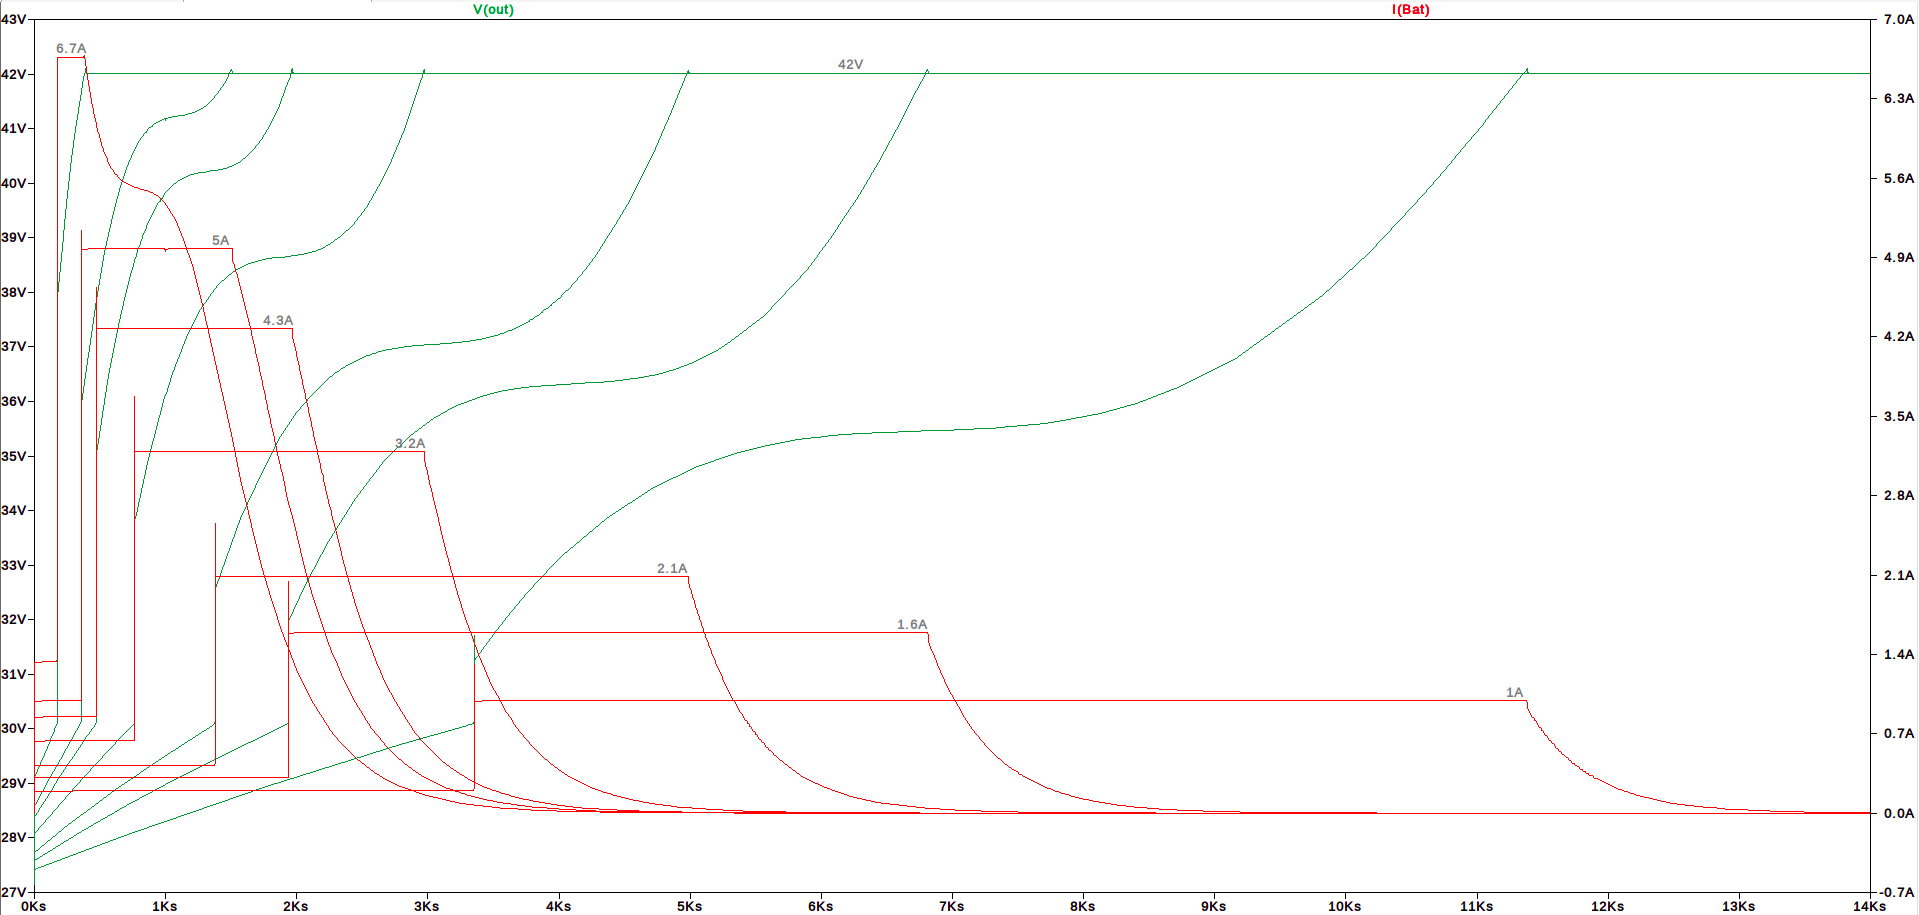
\includegraphics[width=\linewidth]{images/carga_completa_step.png}
    \caption{Simulación de las etapas de carga para todos los modos de corriente}
    \label{fig:simulacion_carga}
\end{figure}
    
\begin{figure}[hbt]
    \centering
    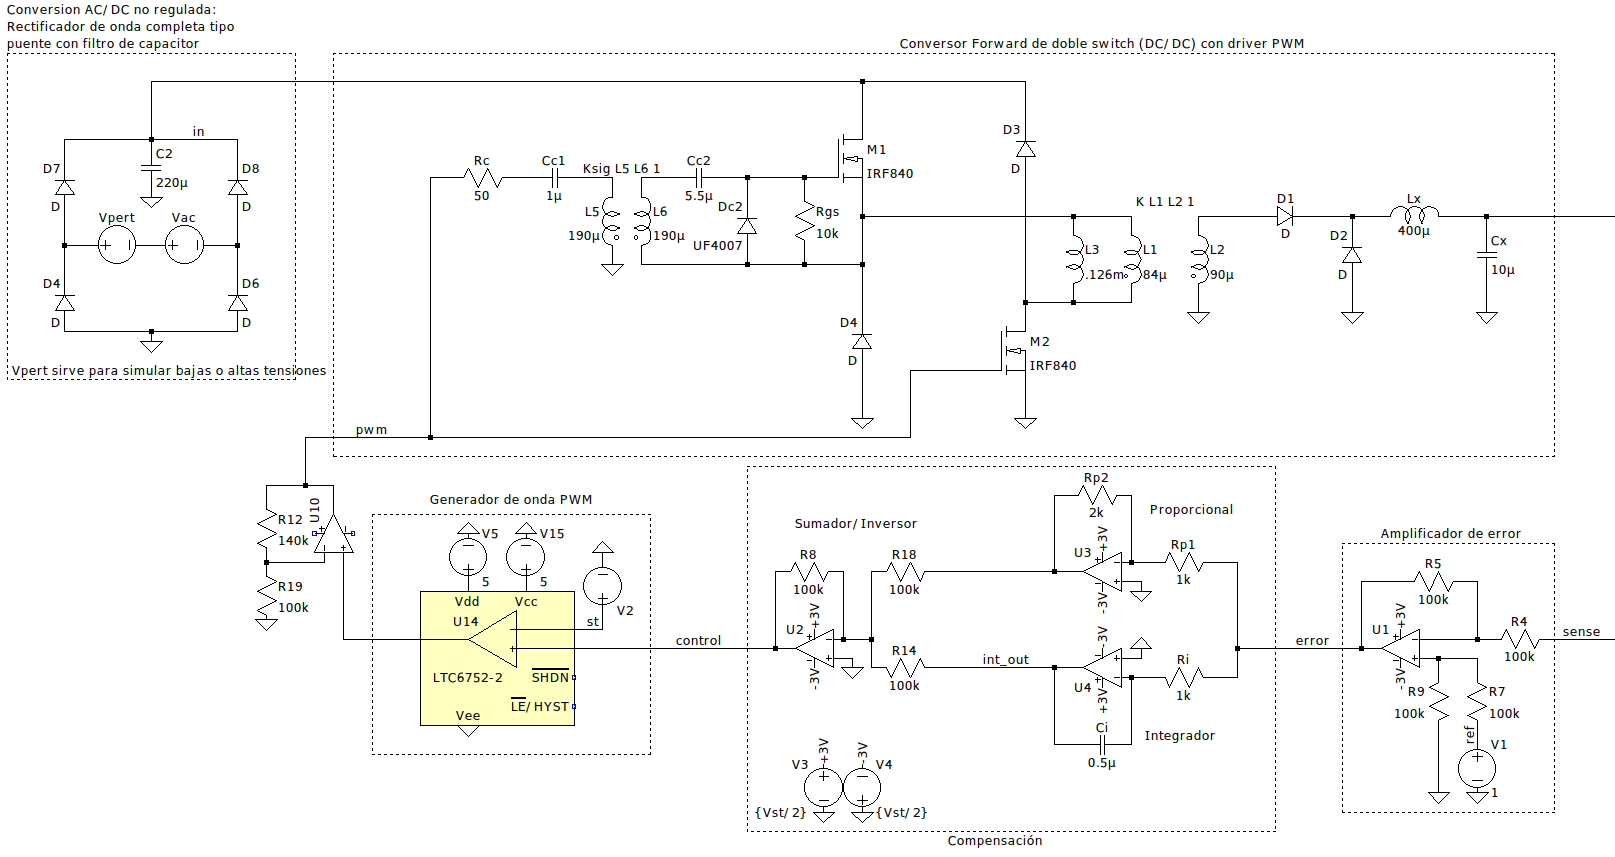
\includegraphics[width=\linewidth]{images/sim-full-1.png}
    \caption{Circuito simulado en LTspice. Se separa cada bloque con línea punteada. Se muestra el recitificador de entrada, el conversor DC-DC y parte del circuito de control.}
    \label{fig:sim-full-1}
\end{figure}

\begin{figure}[hbt]
    \centering
    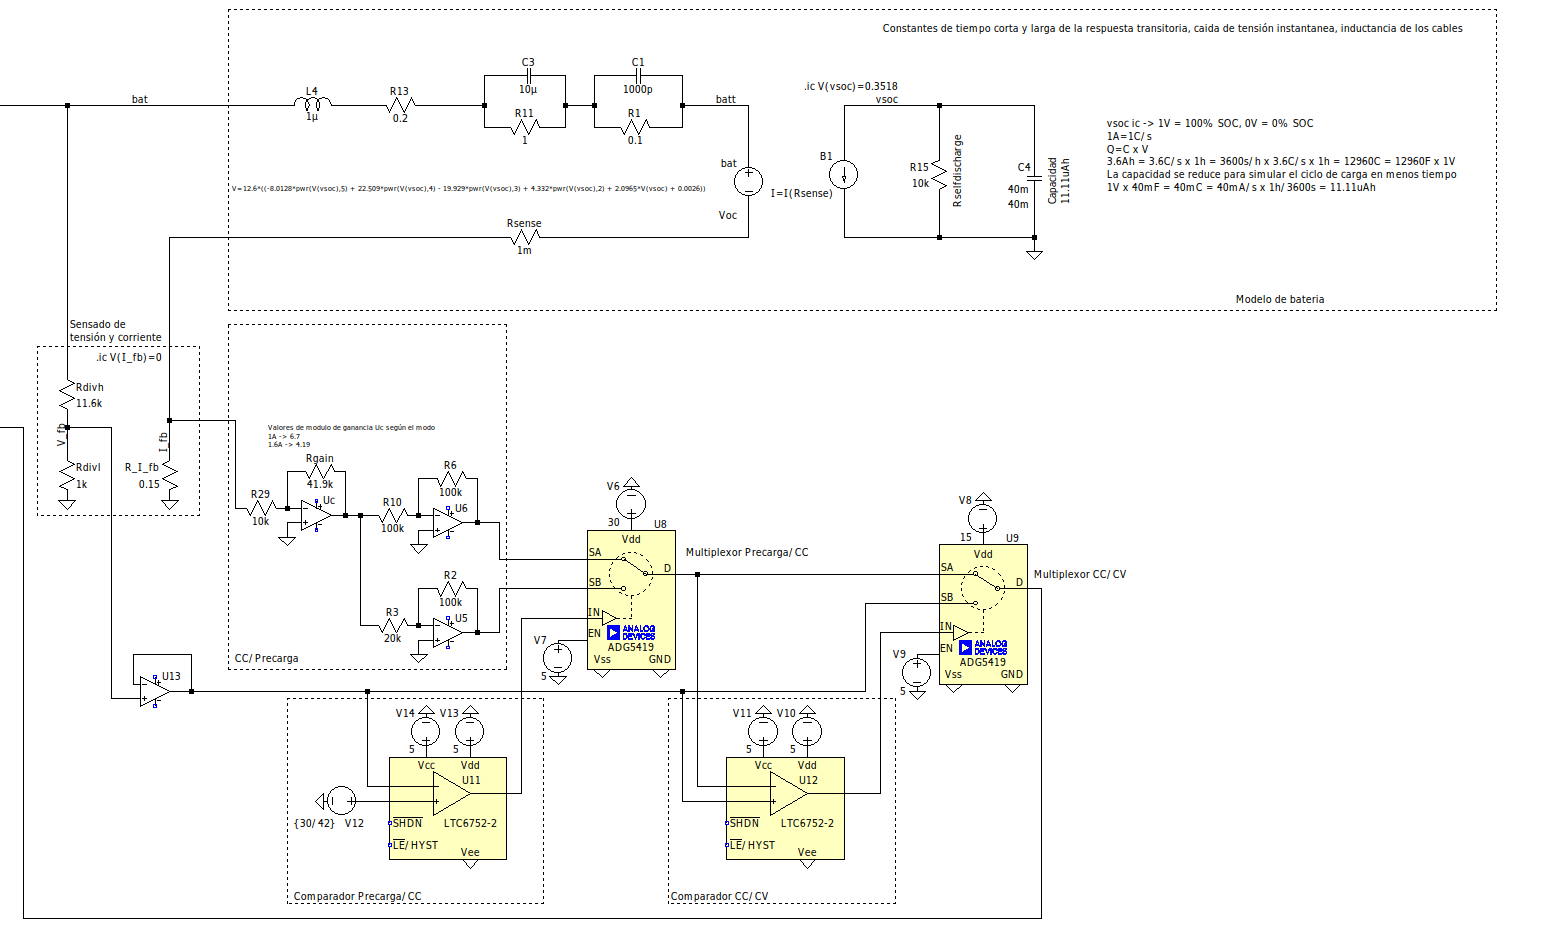
\includegraphics[width=\linewidth]{images/sim-full-2.png}
    \caption{Circuito simulado en LTspice. Se muestra el modelo de batería utilizado y el resto del circuito de control.}
    \label{fig:sim-full-2}
\end{figure}

\begin{figure}[hbt]
    \centering
    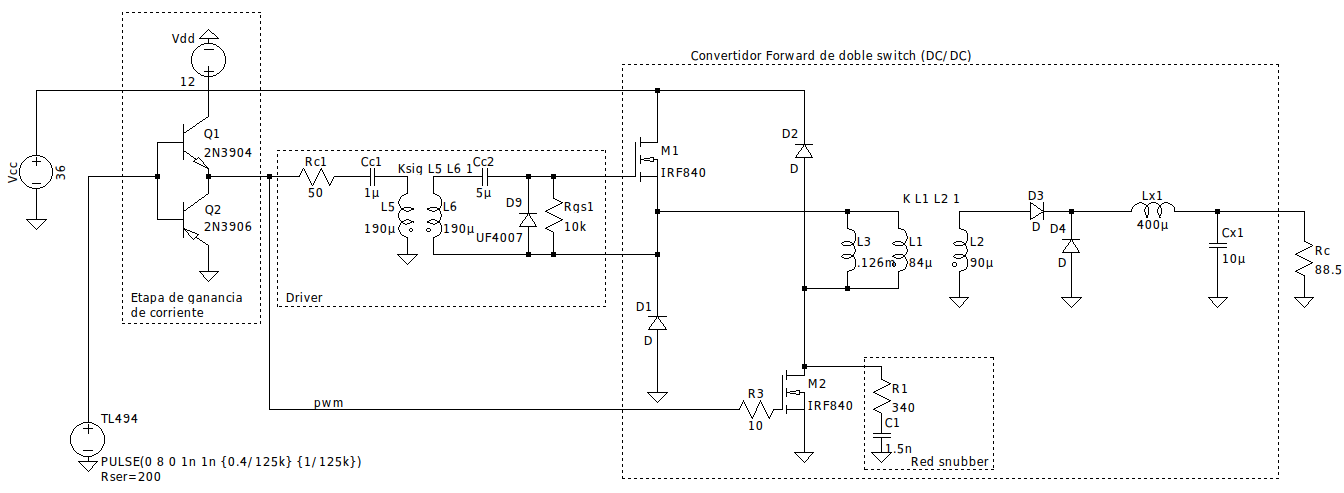
\includegraphics[width=\linewidth]{images/sim-final.png}
    \caption{Circuito final simulado en LTspice}
    \label{fig:sim-final}
\end{figure}

\end{landscape}
\restoregeometry
\newpage
\printbibliography

\end{document}